\ifdefined\included
\else
\setcounter{chapter}{3} %% Numéro du chapitre précédent ;)
\dominitoc
\faketableofcontents
\fi

\chapter{A Task planner making a robot compliant to human online decisions and preferences}
\chaptermark{A Task planner making a robot compliant to human online decisions and preferences}
\label{chap:4}
\minitoc


\section{Introduction}

\section{Related works}
paper Sonia UHTP



\section{Model of Execution}

\subsection{Based on joint action litterature}

\subsection{Model description}

\subsection{Model utility}

\subsection{From Article}

\begin{figure}
    \centering
    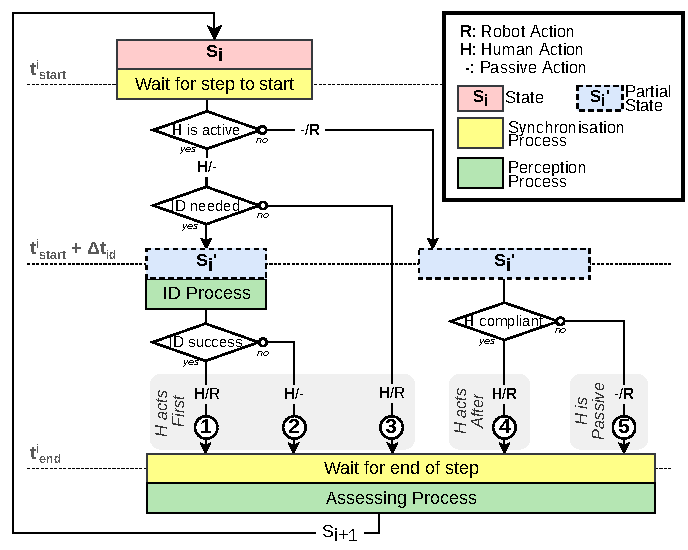
\includegraphics[width=\linewidth]{images/Chapter4/Execution_Automaton.drawio.pdf}
    \caption{
    The Model of Execution, in the form of an automaton and here simplified, captures the latitude of uncontrollable humans in their actions and guides our task planning approach.
    In this paradigm, the two agents can act concurrently but one is always compliant with the other's decision to act.
    Here, the human is always free to decide whether to start acting first, or after the robot, or not to act at all.
    To be compliant, the robot attempts to identify human decisions using perception and situation assessment as well as possible collaborative human signaling acts (e.g., gestures or speech).
    }
    \label{fig:model_of_execution}
\end{figure}

Our task planning approach uses a model of execution to improve the fluency and amenability of HRC. 
This model is in the form of an execution controller as shown in Figure~\ref{fig:model_of_execution}, and is based on several key notions and mechanisms borrowed from studies on joint actions~\cite{Sebanz-2016,kourtis2014attention}, and adapted to Human-Robot Joint Action~\cite{clodic-2017,curioni-2019}.
The key idea is that co-acting agents co-represent the shared task context and integrate task components of their co-actors into their own task representation~\cite{Schmitz-2017, Yamaguchi-19}. Also, coordination and role distribution rely strongly on reciprocal information flow, e.g., social signals~\cite{curioni-2019}, prediction of other's next action~\cite{luke-2018}.

Our proposed execution model is implemented on a robot that co-acts with a human, integrating explicit representation and exploration of the task representations for the robot and for the human. 
It also identifies precisely how reciprocal information flow is used in task execution (detecting and interpreting human actions, signals produced by the robot while acting, and also when the robot waits for human actions or their signals).

Another essential question is the criteria for choosing the next action, or more globally, how to share the load between the two co-actors. The choice depends on the context and actors' preferences~\cite{Gombolay-2015, Strachan-2020,Curioni-2022}. 
Concerning the case when one actor is a robot, we think it is important to provide a standard default behavior of the robot where the robot does its best to reduce human load but still leaves full latitude to act whenever humans want. 
Our scheme provides this ability and also allows humans to inform about their preferences at any moment.

Consider an example to clarify the execution automaton. 
Assume a human and a robot have to pick up two blocks, \textit{A} and \textit{B}, that both can reach. 
They can pick it up both at the same time unless they try to pick up the same block, which causes conflicts between their actions. 
As a result, despite being executable in parallel, the actions are interdependent, and in order to avoid conflicts, one agent must be compliant with the other. 
However, if we consider a third block \textit{C} that only the robot can reach, it can always pick up this block without any risk of conflicts with the human's choice. 

In a state, a human decision can result in one of three outcomes.
First, the human can choose to act first (\textit{left~subtree}).
If the robot's best action is not in conflict with the human action (e.g., \textit{pick~C}), the robot can safely perform this action concurrently with the human operator (\textit{branch~3}).
However, if the robot's best action is either \textit{pick~A} or \textit{pick~B}, the human action must be identified first with a subroutine in order to be compliant with it.
If this subroutine is successful the robot can perform any action which is congruent with the identified human action (\textit{branch~1}). 
This includes the robot's choice to be \textit{passive} and let the human act alone. 
However, if the robot is unable to identify the human action, it must remain passive in order to avoid potential conflicts (\textit{branch~2}). 
Then, the human can either decide to be \textit{passive} or to act after the robot (\textit{right~subtree}). 
In both cases, the human is \textit{passive} at the beginning, making the robot to start performing alone a feasible action. 
While the robot is acting, the human is free to remain \textit{passive} until the next step (\textit{branch~5}), or to choose a congruent action to act concurrently (\textit{branch~4}). 
As a result, the human can always choose to 1) act first, 2) act after the robot, or 3) not act at all. 
The robot will always be compliant with these online human decisions.

When both agents finish their actions, the step is considered as \textit{``over''}. 
Then, another subroutine assesses the new world state ($s_{i+1}$), which is the result of the concurrent actions being executed in the state $s_i$, before repeating the whole process until the task is solved.

Note that if both agents are passive (the human decides to be passive when the robot cannot act) then the step is repeated. 

\section{Exploration}

heavy, Offline

\subsection{compliant pairs}
\subsection{graph, merge state planning state}


\section{Policy generation}
Light, 

\subsection{Human preferences}
estimations, format, Discussion(often inaccurate, hence our Approach)

\subsection{process}
propagation + merge + policy format 

\section{Results}
simulation of execution, without durative action

\subsection{concept of aligned-adversarial pairs of prefs/estimations}

\subsection{results}

\section{Discussion and Limitations}
\section{Conclusion}




